\chapter{Object Versioning} \label{chapter:APPROACH}

When programmers unexpectedly introduce problems to the functionality, performance, or design of their applications, they might want to recover a previous development state.
In programming systems like Lively, where programmers often work at runtime on objects, a development state consists of objects, or, more precise, of the state of objects, which includes object-specific behavior.
To be able to recover such a development state, comprehensive recovery support for Lively must, therefore, preserve versions of objects.

Our approach for this builts upon alternative, version-aware references that manage versions of objects transparently.
That is, objects are pointed to through references that dynamically and transparently choose versions of objects as they were at a particular moment.
When these references are then used for all mutable objects of a runtime, the entire runtime state can be preserved and re-established.

Our concrete solution for implementing this in JavaScript and for the Lively Kernel relies on proxies and source transformations.
Using proxies and source transformations allows a language-level solution for alternative references.
The proxies, in this solution, also contain the versions of the object they stand-in for, enabling the ordinary JavaScript garbage collection to reclaim the versions of an object when the version-aware reference is no longer used.



\section{Version-aware References} \label{sec:APPROACH:1}

For object versioning in systems like Lively, we propose alternative, version-aware references to manage multiple versions of objects.
These version-aware references know the available versions for an object and resolve to one of those.
A version of an object is, in the simplest case, a copy of an object---also an object and also part of the application memory.
That is, a version-aware cencapsulates the multiplicity of different objects for conceptually the same object.

To preserve complete development states, all objects of the programming runtime need to be preserved and accessed via version-aware references.
That is, to save a version of the runtime, versions of all objects are preserved---which also entails that the side effects to the state of other programs, for example server processes, or to databases are not preserved with this approach.
To then re-establish a version of the runtime, the version-aware references all choose versions of objects that were preserved together.
This way, multiple version-aware references can be resolved transitively to the state as it was when the versions were preserved.

Version-aware references behave transparent, like usual references.
They can be assigned to variables and be passed around, and, under usual circumstances, programmers do not have to be aware of them.
Firstly, programmers should not have to adapt their program code to use version-aware references.
Instead version-aware references should be provided consistently by the programming system.
Secondly, there should not be direct references to particular versions of an objects, which otherwise would potentially introduce inconsistencies.
Programmers should not have to distinguish between version-aware references and direct references.

This approach to object versioning allows incremental versioning, without interrupting the system.
The version-aware references resolve dynamically to particular versions based on context information.
Only this context information has to be changed to have all references resolve to another version, without updating any of the version-aware references.
Similarly, preserving a new version of the runtime can also happen incrementally.
Instead of preserving versions of all objects that make up the runtime, new versions of objects are only created when objects change.
Before writes, the previously preserved objects continue to reflect the current state and can, thus, be read for following versions.
This way, versioning happens on the granularity of objects.

\begin{figure}[h]
    \centering
    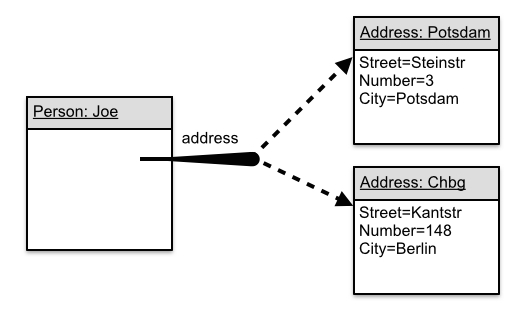
\includegraphics[width=0.5\textwidth]{figures/versionAwareReference.png}
    \caption{A Person object with two versions for its address.}
    \label{fig:VersionAwareReference}
\end{figure}

Figure~\ref{fig:VersionAwareReference} shows a version-aware reference and three objects:
a \emph{Person} object and two different versions of conceptually the same \emph{address} object.
The person holds the version-aware reference to the addresses in its \emph{address} slot.
The version-aware reference can resolve to both, dynamically using context information to decide this matter.
That is, it does not have to have one of the versions hard-wired as active version.

\begin{figure}[h]
    \centering
    \includegraphics[width=\textwidth]{figures/MultipleVersionAwareReferences.png}
    \caption{Three versions visible in the version-aware references of a simple object graph.}
    \label{fig:MoreVersionAwareReferences}
\end{figure}

To resolve entire object graphs to consistent versions and as they have been at particular moments, versions of objects are created and resolved in a coordinated way.
For this example, we assume that the context information that is used to resolve version-aware references, is a global version identifier that corresponds to meta-information stored in the version-aware references, as shown in Figure~\ref{fig:MoreVersionAwareReferences}.
This example shows a slightly more comprehensive graph that might result from preserving specific versions while changing particular objects.
We have an initial version, \emph{v1}.
In this, a \emph{Company} object is created and that refers to a \emph{CEO} object using a version-aware reference.
The CEO in turn has an address, also referred to via a version-aware reference.
Next, we preserve this version and then, in version \emph{v2}, the same CEO moves to Berlin.
Therefore, the version-aware reference to the address of the first CEO knows two different addresses.
Finally, to achieve the situation as shown in the figure, we preserve the second version and, in version \emph{v3} change the company's CEO and this new CEO has its own address.
Now, given the knowledge that \emph{v3} is preceded by \emph{v2} and that by \emph{v1}, the version-aware references can resolve to three different development states the runtime was in.
When, for example, changing the CEO turns out to be a mistake, we can re-establish \emph{v2} and, therefore, the old CEO with its address in Berlin.
This way, when version-aware references are used consistently for all object relations in a programming runtime, the state of the entire runtime can be set to particular versions.

What versions of the runtime get preserved is not inherent to our approach, but can be different for different use cases.
Programmers could, as described in the second example, explicitly preserve versions or the programming system could implicitly preserve versions.
For example, each manipulating user interaction could yield a new version of the runtime.
Such actions could include directly manipulating attributes and composition of graphical elements, saving source code, evaluating do-its, and, for example, firing buttons of applications.
This way, programmers could undo each of their actions, regardless of whether the action was intended as mere exploration or turned out inappropriate more unexpectedly.
Using user actions as granularity also allows developers to undo and redo the changes associated with specific and rememberable actions.
The resulting histories can be fine-grained as for each version only changed objects need to be copied.
For the same reason, creating many versions is not expected to be problematic for the development workflow.
In general, the approach distributes the cost for object versioning: besides incrementally saving a version, switching the active version is also not interruptive.



\section{Object Versioning for the Lively Kernel} \label{sec:APPROACH:2}

Our approach for providing object versioning for the Lively Kernel uses proxies to implement version-aware references in JavaScript.
We exchange ordinary references with proxies for all mutable objects by returning proxies whenever a new object is created.
This is done by transforming sources to proxy object literals and constructor functions.
Further, the proxies return proxies again when they are used as constructors.
Also through proxy behavior and some global versioning data, we provide basic recovery support for the single-threaded Lively Kernel programming system.


\subsection{Proxies as Version-aware References}

We do not actually require an alternative kind of references for JavaScript to provide version-aware references.
Instead we can use ordinary references and proxy objects.
That is, each reference that would normally point directly to an object points to a proxy instead.
The proxies know how to access the actual versions for each object and delegate transparently to one particular among those.

we let the proxy objects hold all versions of an object instead of, for example, using object tables, so that when no object holds the version-aware reference any longer, the proxy object and all actual version objects get garbage collected.

fully virtual objects, intercept all kinds of access to the proxies and can handle that access arbitrarly.
our implementation delegates intercepted to the current version.

%  ECMAScript 6 Direct Proxies: fully virtual objects, traps to specify proxy behavior, traps for property reads, property writes, accessing the prototype, other meta programming... where we delegate each of those actions to the current version


\subsection{Proxies For All Mutable Objects}

This ensures that references to proxies are used consistently instead of direct references to objects and that such proxies are used for every object.

for all references that would normally relate two objects we need version-aware references instead.
that is, all usual references need to become references to proxy objects, which then reference one or multiple versions of the actual object.
also, two references to the same proxy object have to be identical as references to the same object are identical.
for this reason, we create a proxy as an object is created and return a reference to the proxy instead to the object.
this reference to the proxy is, thus, then passed around in the program as only access to the versioned object.
therefore, all access goes through the proxy and there are no direct references to the object.
further, identity that would usually compare the object with other objects now compares the proxy with other proxies.

for our approach, all expressions that create new objects need to return proxies for those objects instead.
there are three different ways to create an object in javascript: evaluating literal expressions, applying constructor functions, and calling specific built-in functions as, for example, the eval function.

we apply source transformation to wrap literal expressions in a function that creates and returns a proxy for the expression's result.
besides objects and arrays functions are also mutable objects in javascript.
therefore, we wrap the literal forms of objects, arrays, and functions.

in javascript, all functions can be constructors and create new objects when called with the new operator.
except, for built-in functions of JavaScript standard library all functions are expressed as function literals, which we transform to be wrapped by our proxies.
as the virtual object proxies we use for version-aware references intercept different object access differently, we can specify their construct behavior and let them return proxies for the newly created objects.

however, there are also built-in functions that create objects and that are not created from literal form.
therefore, these are not automatically proxied.
one category of such built-in functions are built-in constructors.
for example, the built-in data types like objects and arrays can be created by calling new Object or new Array.
we transform these built-in constructor functions explicity, wrapping each into the proxying function.
besides this category, there are also very specific built-in functions, that we transform separately to specific alternatives.
one example for such functions is the global eval function.
while the return value of that function also potentially needs to be a reference to a proxy instead of an ordinary object, eval takes arbitrary code which might express an arbitrary object structure where references also should not be directly between objects.
therefore, in the case of eval, we wrap eval, but also let the string argument to eval pass through our source transformations.


\subsection{Versions of the Lively Runtime}

developers can only effectively undo changes, which potentially affect many objects and are not necessarily fully known, when whole object graphs or even the entire runtime can be re-set to a particular state.
for this, the version-aware references for multiple objects need to resolve to versions that were saved together.
therefore, our proxies hold all versions for an object in a dictionary that connects version identifiers for actual objects.
which of these versions for each object should be chosen can be declared globally as javascript runs single-threaded and with cooperative scheduling and there is, thus, no possiblity to cause inconsistencies through accidentaly changing the global version within JavaScript while another JavaScript function is executed.
this global versioning information is an object that holds a version identifier, to be used by the proxies when deciding to which version they delegate, and may also have a predecessor and a successor.

this global versioning information with its potentially predecessor and successor can also be used to not copy every object for every preserved state of the runtime.
that is, when an object has not changed from one version to the next, it does not need to be copied.
the version-aware references could just follow the global information to return the last preserved version.

besides this copy-on-write optimization, another optimization would be to not copy objects completely, but to only store changes.
this could, for example, also apply prototypical inheritance to have versions that delegate to previous versions and only express the differences between versions.